\documentclass[tikz,border=6pt]{standalone}
\usepackage{amsmath,amssymb}
\usepackage{xcolor}
\definecolor{accent}{HTML}{A13D2C}
\definecolor{accent2}{HTML}{2B5F6B}
\definecolor{muted}{HTML}{5A564F}
\definecolor{panel}{HTML}{F8F6F0}
\definecolor{linecol}{HTML}{D8D2C4}
\definecolor{astroblue}{HTML}{1B4F72}
\definecolor{ink}{HTML}{1E1C1A}
\usetikzlibrary{calc,arrows.meta}
\usepackage[T1]{fontenc}\usepackage{newpxtext,newpxmath}  % same fonts as the notes
\begin{document}
% Active nuclei as a tree: one engine (an accreting supermassive black hole), sorted first by whether it has a
% strong jet, then by luminosity (no jet) or by the angle between the jet and our sight line (jet).
% Leaves name the kind and say what is seen, as in the table "Kinds of active galaxies" of the chapter.
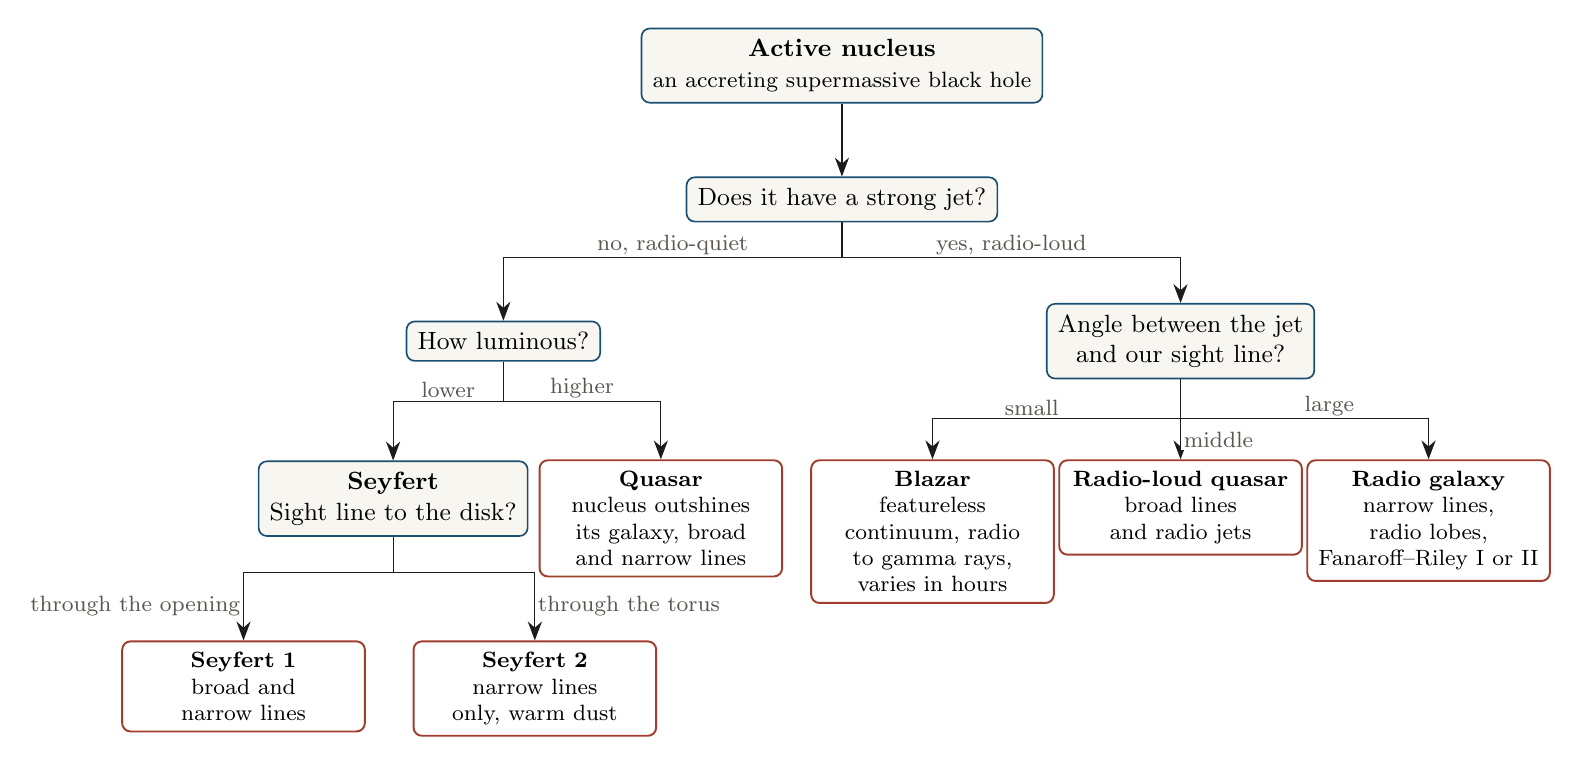
\begin{tikzpicture}[font=\small, >={Stealth[length=2.4mm]},
  q/.style={draw=astroblue, line width=0.6pt, fill=panel, rounded corners=3pt, align=center, inner sep=4pt},
  leaf/.style={draw=accent, line width=0.7pt, fill=white, rounded corners=3pt, align=center, text width=2.8cm, inner sep=4pt, font=\footnotesize, execute at begin node={\hyphenpenalty=10000\exhyphenpenalty=10000}},
  lab/.style={muted, font=\footnotesize, fill=white, inner sep=1pt}]
  \node[q] (root) at (0,0) {\textbf{Active nucleus}\\ \footnotesize an accreting supermassive black hole};
  \node[q] (jet) at (0,-1.7) {Does it have a strong jet?};
  \node[q] (lum) at (-4.3,-3.5) {How luminous?};
  \node[q] (ang) at (4.3,-3.5) {Angle between the jet\\ and our sight line?};
  \node[q] (sey) at (-5.7,-5.5) {\textbf{Seyfert}\\ Sight line to the disk?};
  \node[leaf, anchor=north] (qso) at (-2.3,-5.0) {\textbf{Quasar}\\ nucleus outshines its galaxy, broad and narrow lines};
  \node[leaf, anchor=north] (s1) at (-7.6,-7.3) {\textbf{Seyfert 1}\\ broad and narrow lines};
  \node[leaf, anchor=north] (s2) at (-3.9,-7.3) {\textbf{Seyfert 2}\\ narrow lines only, warm dust};
  \node[leaf, anchor=north] (bla) at (1.15,-5.0) {\textbf{Blazar}\\ featureless continuum, radio to gamma rays, varies in hours};
  \node[leaf, anchor=north] (rlq) at (4.3,-5.0) {\textbf{Radio-loud quasar}\\ broad lines and radio jets};
  \node[leaf, anchor=north] (rg) at (7.45,-5.0) {\textbf{Radio galaxy}\\ narrow lines, radio lobes, \mbox{Fanaroff--Riley} I or II};
  \draw[ink, ->] (root) -- (jet);
  \draw[ink, ->] (jet.south) -- ++(0,-0.45) -| node[lab, pos=0.25, above] {no, radio-quiet} (lum.north);
  \draw[ink, ->] (jet.south) -- ++(0,-0.45) -| node[lab, pos=0.25, above] {yes, radio-loud} (ang.north);
  \draw[ink, ->] (lum.south) -- ++(0,-0.5) -| node[lab, pos=0.25, above] {lower} (sey.north);
  \draw[ink, ->] (lum.south) -- ++(0,-0.5) -| node[lab, pos=0.25, above] {higher} (qso.north);
  \draw[ink, ->] (sey.south) -- ++(0,-0.45) -| node[lab, pos=0.75, left] {through the opening} (s1.north);
  \draw[ink, ->] (sey.south) -- ++(0,-0.45) -| node[lab, pos=0.75, right] {through the torus} (s2.north);
  \draw[ink, ->] (ang.south) -- ++(0,-0.5) -| node[lab, pos=0.3, above] {small} (bla.north);
  \draw[ink, ->] (ang.south) -- node[lab, right, pos=0.75] {middle} (rlq.north);
  \draw[ink, ->] (ang.south) -- ++(0,-0.5) -| node[lab, pos=0.3, above] {large} (rg.north);
\end{tikzpicture}
\end{document}
